%% Patent Application: Method for Verifying Resonant Protein Folding Modulation
%% Using Isotope Substitution
%% Inventor: Jonathan Washburn
%% Contact: washburn.jonathan@gmail.com
%% Filing Date: January 2026

\documentclass[12pt,letterpaper]{article}

\usepackage[margin=1in]{geometry}
\usepackage{amsmath,amssymb,amsfonts}
\usepackage{graphicx}
\usepackage{tikz}
\usetikzlibrary{shapes,arrows,positioning,calc,patterns,decorations.pathmorphing}
\usepackage{booktabs}
\usepackage{array}
\usepackage{enumitem}
\usepackage{fancyhdr}
\usepackage{xcolor}
\usepackage{hyperref}
\usepackage{setspace}

% Patent-style formatting
\setlength{\parindent}{0.5in}
\setlength{\parskip}{0.5em}
\onehalfspacing

% Header
\pagestyle{fancy}
\fancyhf{}
\rhead{Patent Application}
\lhead{Washburn}
\rfoot{Page \thepage}

\hypersetup{
    colorlinks=true,
    linkcolor=blue,
    urlcolor=blue,
    citecolor=blue
}

% Custom colors
\definecolor{h2o}{RGB}{50,100,200}
\definecolor{d2o}{RGB}{200,80,80}
\definecolor{thermal}{RGB}{150,150,150}

\begin{document}

%% ============================================================================
%%                              TITLE PAGE
%% ============================================================================

\begin{center}
\vspace*{0.8in}

{\LARGE \textbf{PATENT APPLICATION}}

\vspace{0.4in}

{\Large \textbf{METHOD FOR VERIFYING RESONANT}}

{\Large \textbf{PROTEIN FOLDING MODULATION}}

{\Large \textbf{USING ISOTOPE SUBSTITUTION}}

\vspace{0.8in}

\textbf{PROVISIONAL PATENT APPLICATION}

\vspace{0.5in}

\begin{tabular}{ll}
\textbf{Inventor:} & Jonathan Washburn \\
\textbf{Email:} & washburn.jonathan@gmail.com \\
\textbf{Filing Date:} & January 17, 2026 \\
\textbf{Application Type:} & Utility Patent (Provisional) \\
\textbf{Related Applications:} & Patent 001 (Method), Patent 002 (Apparatus) \\
\end{tabular}

\vspace{0.8in}

\textit{A method for unambiguously verifying that modulation of protein folding rates by microwave irradiation is due to a resonant mechanism rather than thermal heating, using the characteristic $\sqrt{2}$ isotope shift between H$_2$O and D$_2$O as a diagnostic signature.}

\vfill

\textbf{CONFIDENTIAL --- PATENT PENDING}

\end{center}

\newpage

%% ============================================================================
%%                         TABLE OF CONTENTS
%% ============================================================================

\tableofcontents
\newpage

%% ============================================================================
%%                              ABSTRACT
%% ============================================================================

\section*{ABSTRACT OF THE DISCLOSURE}
\addcontentsline{toc}{section}{ABSTRACT OF THE DISCLOSURE}

A method for verifying that modulation of protein folding rates by electromagnetic radiation is due to a resonant mechanism coupling to molecular gating dynamics, rather than bulk thermal heating. The method comprises: (a) performing a first measurement of protein folding rate modulation in aqueous (H$_2$O) solution at a first frequency $f_1$ in the range of 12--17 GHz; (b) performing a second measurement in deuterated water (D$_2$O) at a second frequency $f_2 = f_1/\sqrt{2}$, corresponding to the range 8--13 GHz; (c) comparing the magnitude of folding rate modulation at the two frequencies; and (d) confirming a resonant mechanism if the modulation magnitudes are equal within experimental uncertainty. The $\sqrt{2}$ isotope shift arises from the mass dependence of the molecular gate oscillation frequency ($\omega \propto 1/\sqrt{m}$) and cannot arise from bulk thermal effects, which would show at most a $\sim$10\% shift due to different dielectric properties. The method provides a ``smoking gun'' signature for the resonant mechanism predicted by Recognition Science, enabling unambiguous discrimination between resonant and thermal effects in any experimental system. Machine-verified proofs establish that the H$_2$O jamming frequency lies in (12, 17) GHz and the D$_2$O frequency lies in (8, 13) GHz, with ratio $\sqrt{2}$.

\vspace{1em}
\noindent\textbf{Keywords:} isotope effect, deuterium oxide, resonant verification, protein folding, microwave irradiation, molecular gate, thermal discrimination

\newpage

%% ============================================================================
%%                      BACKGROUND OF THE INVENTION
%% ============================================================================

\section{BACKGROUND OF THE INVENTION}

\subsection{Field of the Invention}

The present invention relates generally to methods for characterizing the mechanism of electromagnetic effects on biological systems, and more specifically to methods for distinguishing resonant from thermal effects in microwave modulation of protein folding using isotope substitution experiments.

\subsection{Description of Related Art}

\subsubsection{The Thermal vs.\ Resonant Controversy}

A longstanding controversy in biophysics concerns whether electromagnetic effects on biological systems are predominantly thermal (arising from bulk heating due to dielectric absorption) or non-thermal/resonant (arising from specific coupling to molecular motions). This controversy has significant implications for:

\begin{enumerate}[label=(\alph*)]
\item \textbf{Therapeutic applications:} If effects are purely thermal, microwave therapy offers no advantage over conventional heating. If effects are resonant, specific frequencies may have specific biological activities.

\item \textbf{Safety standards:} Thermal effects can be predicted from specific absorption rate (SAR) and managed by temperature control. Resonant effects may occur at power levels too low to cause measurable heating.

\item \textbf{Mechanism understanding:} Thermal effects are well-understood via classical thermodynamics. Resonant effects would require new theoretical frameworks.
\end{enumerate}

\subsubsection{Prior Approaches to Distinguishing Thermal from Non-Thermal Effects}

Several approaches have been used to address this controversy:

\begin{enumerate}[label=(\arabic*)]
\item \textbf{Temperature monitoring:} Measuring sample temperature during irradiation. \textit{Limitation:} Local heating may occur even if bulk temperature is constant; thermal equilibration may be faster than measurement resolution.

\item \textbf{Power dependence:} Comparing effects at different power levels. \textit{Limitation:} Both thermal and resonant effects may scale with power, just with different functional forms.

\item \textbf{Frequency dependence:} Scanning frequency to look for resonances. \textit{Limitation:} Thermal absorption also varies with frequency (dielectric dispersion); resonances may be broad and difficult to distinguish.

\item \textbf{Comparison with conventional heating:} Comparing microwave effects with effects of equivalent conventional heating. \textit{Limitation:} Heating profiles (spatial and temporal) may differ, confounding comparison.

\item \textbf{Pulsed irradiation:} Using short pulses to minimize heating. \textit{Limitation:} Does not definitively prove non-thermal mechanism.
\end{enumerate}

\subsubsection{Limitations of Prior Art}

None of the prior approaches provides an unambiguous ``smoking gun'' signature for distinguishing resonant from thermal mechanisms:

\begin{table}[h]
\centering
\begin{tabular}{p{0.3\textwidth}p{0.6\textwidth}}
\toprule
\textbf{Prior Approach} & \textbf{Why Not Definitive} \\
\midrule
Temperature monitoring & Local heating may be missed; thermal equilibration may mask transients \\
\addlinespace
Power dependence & Both mechanisms scale with power \\
\addlinespace
Frequency scanning & Dielectric dispersion creates frequency-dependent thermal effects \\
\addlinespace
Conventional heating comparison & Different heating profiles confound comparison \\
\addlinespace
Pulsed irradiation & Does not rule out rapid thermal effects \\
\bottomrule
\end{tabular}
\caption{Limitations of prior approaches to thermal/resonant discrimination}
\end{table}

\subsubsection{The Need for a Definitive Test}

What is needed is a test that:

\begin{enumerate}[label=(\arabic*)]
\item Provides a \textbf{quantitative prediction} that differs between thermal and resonant mechanisms;
\item Is based on \textbf{first principles} rather than empirical fitting;
\item Can be \textbf{independently verified} without specialized equipment;
\item Provides an \textbf{unambiguous signature} that cannot arise from thermal effects.
\end{enumerate}

\subsection{The Isotope Shift Solution}

\subsubsection{Physical Basis}

The present invention exploits a fundamental difference between thermal and resonant mechanisms in their response to isotope substitution:

\begin{enumerate}[label=(\alph*)]
\item \textbf{Resonant mechanism:} If microwave radiation couples to a specific molecular oscillation, the resonant frequency depends on the effective mass of the oscillating component:
\begin{equation}
\omega = \sqrt{\frac{k}{m}} \quad \Rightarrow \quad f \propto \frac{1}{\sqrt{m}}
\label{eq:oscillator}
\end{equation}
When hydrogen (H) is replaced by deuterium (D), the mass doubles, so the frequency shifts by factor $1/\sqrt{2}$.

\item \textbf{Thermal mechanism:} Bulk heating depends on the dielectric absorption of the solvent. The dielectric properties of H$_2$O and D$_2$O differ by only $\sim$10\% in the relevant frequency range, so thermal effects would show at most a $\sim$10\% frequency shift.
\end{enumerate}

\subsubsection{The $\sqrt{2}$ Signature}

The $\sqrt{2}$ ($\approx 1.414$) frequency shift upon H$_2$O $\to$ D$_2$O substitution is a unique signature of the resonant mechanism:

\begin{table}[h]
\centering
\begin{tabular}{lcc}
\toprule
\textbf{Mechanism} & \textbf{Predicted Frequency Shift} & \textbf{Shift Magnitude} \\
\midrule
Resonant (present invention) & $f_{\text{D}_2\text{O}} = f_{\text{H}_2\text{O}} / \sqrt{2}$ & $\sim$41\% \\
Thermal (dielectric) & $f_{\text{D}_2\text{O}} \approx 0.9 \times f_{\text{H}_2\text{O}}$ & $\sim$10\% \\
\bottomrule
\end{tabular}
\caption{Predicted frequency shifts for resonant vs.\ thermal mechanisms}
\end{table}

The 41\% shift (resonant) is clearly distinguishable from the $\sim$10\% shift (thermal), providing an unambiguous diagnostic.

\subsection{Objects of the Invention}

It is an object of the present invention to provide a method for:

\begin{enumerate}[label=(\arabic*)]
\item Unambiguously distinguishing resonant from thermal mechanisms in microwave effects on protein folding;
\item Verifying that observed effects are due to coupling to molecular gate dynamics;
\item Providing a quantitative, falsifiable prediction that can be tested experimentally;
\item Enabling validation of the Recognition Science framework for protein folding modulation.
\end{enumerate}

\newpage

%% ============================================================================
%%                      SUMMARY OF THE INVENTION
%% ============================================================================

\section{SUMMARY OF THE INVENTION}

\subsection{General Statement of the Invention}

The present invention provides a method for verifying that modulation of protein folding rates by microwave irradiation is due to a resonant mechanism, comprising:

\begin{enumerate}[label=(\alph*)]
\item Performing a first measurement of folding rate modulation in H$_2$O at a first frequency $f_1$;
\item Performing a second measurement in D$_2$O at a second frequency $f_2 = f_1/\sqrt{2}$;
\item Comparing the magnitudes of folding rate modulation;
\item Confirming a resonant mechanism if modulations are equal within experimental uncertainty.
\end{enumerate}

\subsection{The Verification Protocol}

\subsubsection{Step 1: H$_2$O Measurement}

Prepare a protein sample in H$_2$O buffer and irradiate at frequency $f_1$ in the range 12--17 GHz. The preferred frequency is $f_1 \approx 14.65$ GHz, corresponding to the predicted jamming frequency. Measure the folding rate $k_1$ and compare to an unirradiated control to determine the modulation magnitude:

\begin{equation}
M_1 = \frac{k_{\text{control}} - k_1}{k_{\text{control}}} \times 100\%
\label{eq:modulation_h2o}
\end{equation}

\subsubsection{Step 2: D$_2$O Measurement}

Prepare an identical protein sample in D$_2$O buffer and irradiate at frequency:

\begin{equation}
f_2 = \frac{f_1}{\sqrt{2}} \approx 0.7071 \times f_1
\label{eq:f2}
\end{equation}

For $f_1 = 14.65$ GHz, this gives $f_2 \approx 10.4$ GHz. Measure the folding rate $k_2$ and determine modulation:

\begin{equation}
M_2 = \frac{k_{\text{control,D}_2\text{O}} - k_2}{k_{\text{control,D}_2\text{O}}} \times 100\%
\label{eq:modulation_d2o}
\end{equation}

\subsubsection{Step 3: Comparison}

Compare the modulation magnitudes $M_1$ and $M_2$:

\begin{itemize}
\item If $|M_1 - M_2| < \delta$ (where $\delta$ is the experimental uncertainty), the resonant mechanism is confirmed.
\item If $|M_1 - M_2| > 3\delta$, the resonant mechanism is falsified.
\end{itemize}

\subsubsection{Step 4: Frequency Ratio Verification}

Additionally, verify that the frequency ratio matches the predicted value:

\begin{equation}
\text{Ratio} = \frac{f_1}{f_2} = \sqrt{2} \pm 5\%
\label{eq:ratio}
\end{equation}

If the optimal frequencies in H$_2$O and D$_2$O are independently determined (by frequency sweeps), their ratio should equal $\sqrt{2}$ within experimental uncertainty.

\subsection{Machine-Verified Predictions}

The frequency predictions underlying this method have been formally verified using the Lean 4 theorem prover:

\begin{table}[h]
\centering
\begin{tabular}{lll}
\toprule
\textbf{Theorem} & \textbf{Statement} & \textbf{Lean Proof} \\
\midrule
H$_2$O jamming frequency & $f_{\text{jam}} \in (12, 17)$ GHz & \texttt{direct\_jamming\_approx} \\
D$_2$O jamming frequency & $f_{\text{jam}}^{\text{D}_2\text{O}} \in (8, 13)$ GHz & \texttt{d2o\_jamming\_approx} \\
Frequency ratio & $f_{\text{H}_2\text{O}} / f_{\text{D}_2\text{O}} = \sqrt{2}$ & \texttt{isotope\_shift\_sqrt2} \\
Rung 19 uniqueness & $\tau_{19}$ unique in 50--100 ps & \texttt{rung19\_unique} \\
\bottomrule
\end{tabular}
\caption{Machine-verified frequency predictions}
\end{table}

\subsection{Falsifiability}

The method provides a falsifiable prediction: if the observed optimal frequencies in H$_2$O and D$_2$O do not differ by factor $\sqrt{2}$, or if equal modulation is not observed at $f_1$ and $f_2 = f_1/\sqrt{2}$, the resonant mechanism is falsified.

\newpage

%% ============================================================================
%%                    BRIEF DESCRIPTION OF DRAWINGS
%% ============================================================================

\section{BRIEF DESCRIPTION OF DRAWINGS}

\subsection*{Figure 1: Resonant vs.\ Thermal Frequency Shift}
A diagram comparing the predicted frequency shifts for resonant ($\sqrt{2}$) and thermal ($\sim$1.1) mechanisms.

\subsection*{Figure 2: Verification Protocol Flowchart}
A flowchart showing the steps of the isotope verification protocol.

\subsection*{Figure 3: Expected Resonance Curves}
Predicted resonance curves (folding rate vs.\ frequency) for H$_2$O and D$_2$O samples.

\subsection*{Figure 4: Decision Matrix}
A decision matrix for interpreting experimental results.

\subsection*{Figure 5: Frequency Sweep Comparison}
Expected results of frequency sweeps in H$_2$O and D$_2$O.

\newpage

%% ============================================================================
%%                      DETAILED DESCRIPTION
%% ============================================================================

\section{DETAILED DESCRIPTION OF THE PREFERRED EMBODIMENTS}

\subsection{Theoretical Foundation}

\subsubsection{The Molecular Gate Oscillation}

The resonant protein folding modulation method (described in related Patent Application 001) is based on coupling to the molecular gate---the conformational transition of backbone dihedral angles that governs protein folding dynamics. The characteristic timescale of this gate is:

\begin{equation}
\tau_{19} = \tau_0 \times \varphi^{19} \approx 68 \text{ ps}
\label{eq:tau19}
\end{equation}

where $\varphi = (1+\sqrt{5})/2$ is the golden ratio and $\tau_0$ is a fundamental timescale. The corresponding frequency is:

\begin{equation}
f_{\text{jam}} = \frac{1}{\tau_{19}} \approx 14.65 \text{ GHz}
\label{eq:fjam}
\end{equation}

\subsubsection{Origin of the Isotope Effect}

The molecular gate involves the motion of hydrogen atoms in hydrogen bonds and backbone N-H and C-H bonds. When hydrogen is replaced by deuterium:

\begin{enumerate}[label=(\arabic*)]
\item The mass of the oscillating unit increases by factor $\sim$2.
\item The force constant (bond stiffness) remains unchanged.
\item The oscillation frequency scales as $\omega \propto 1/\sqrt{m}$.
\item Therefore, $f_{\text{D}} = f_{\text{H}} / \sqrt{2}$.
\end{enumerate}

This is the classical isotope effect for harmonic oscillators.

\subsubsection{Why $\sqrt{2}$ and Not 2?}

Although the atomic mass of deuterium (2.014 u) is approximately twice that of hydrogen (1.008 u), the frequency scales with the \textit{square root} of mass, not mass itself:

\begin{equation}
\frac{f_{\text{H}}}{f_{\text{D}}} = \sqrt{\frac{m_{\text{D}}}{m_{\text{H}}}} = \sqrt{\frac{2.014}{1.008}} \approx \sqrt{2} \approx 1.414
\label{eq:sqrt2}
\end{equation}

This $\sqrt{2}$ factor is a fundamental consequence of oscillator physics and provides the basis for the verification method.

\subsubsection{Why Thermal Effects Don't Show $\sqrt{2}$ Shift}

Thermal heating from microwave absorption depends on the dielectric properties of the solvent. Comparing H$_2$O and D$_2$O:

\begin{table}[h]
\centering
\begin{tabular}{lccc}
\toprule
\textbf{Property} & \textbf{H$_2$O} & \textbf{D$_2$O} & \textbf{Ratio} \\
\midrule
Static dielectric constant ($\varepsilon_s$) & 80.1 & 78.1 & 0.975 \\
High-frequency dielectric ($\varepsilon_\infty$) & 4.2 & 4.0 & 0.95 \\
Relaxation time at 25$^\circ$C & 8.3 ps & 10.4 ps & 1.25 \\
Frequency of max loss & 19 GHz & 15 GHz & 0.79 \\
\bottomrule
\end{tabular}
\caption{Dielectric properties of H$_2$O and D$_2$O}
\end{table}

The dielectric properties differ by 5--25\%, corresponding to potential frequency shifts of at most 25\%---far less than the 41\% ($\sqrt{2}$) shift predicted for the resonant mechanism.

\subsection{Detailed Protocol}

\subsubsection{Sample Preparation}

\paragraph{H$_2$O Sample:}
\begin{enumerate}[label=(\arabic*)]
\item Prepare protein at concentration 0.1--10 mg/mL in aqueous buffer (e.g., 20 mM Tris-HCl, pH 7.4).
\item Denature protein by appropriate method (urea, GdnHCl, temperature, or pH jump).
\item Dilute into folding buffer to initiate folding.
\item Load into sample chamber at controlled temperature (typically 20--37$^\circ$C).
\end{enumerate}

\paragraph{D$_2$O Sample:}
\begin{enumerate}[label=(\arabic*)]
\item Exchange protein into D$_2$O buffer by repeated concentration/dilution (at least 3 cycles) or dialysis against D$_2$O buffer.
\item Verify $>$95\% H/D exchange (optional: by mass spectrometry).
\item Prepare matching D$_2$O folding buffer.
\item Follow same denaturation and folding initiation protocol as H$_2$O.
\end{enumerate}

\paragraph{Important Considerations:}
\begin{itemize}
\item pH$_{\text{D}}$ should be set to pD = pH + 0.4 (glass electrode correction).
\item D$_2$O slightly stabilizes proteins; account for this in control measurements.
\item Temperature should be matched precisely (D$_2$O has slightly different thermal properties).
\end{itemize}

\subsubsection{Frequency Selection}

\paragraph{Method A: Fixed Frequencies}

Use the theoretically predicted frequencies:
\begin{align}
f_1 &= 14.65 \text{ GHz (H$_2$O)} \\
f_2 &= 10.37 \text{ GHz (D$_2$O)}
\end{align}

\paragraph{Method B: Optimized Frequencies}

Determine optimal frequencies empirically:
\begin{enumerate}[label=(\arabic*)]
\item Perform frequency sweep in H$_2$O from 12 to 17 GHz.
\item Identify frequency $f_1^*$ of maximum folding rate reduction.
\item Perform frequency sweep in D$_2$O from 8 to 13 GHz.
\item Identify frequency $f_2^*$ of maximum folding rate reduction.
\item Verify that $f_1^*/f_2^* = \sqrt{2} \pm 5\%$.
\end{enumerate}

Method B provides additional confirmation by independently determining both optimal frequencies.

\subsubsection{Irradiation Protocol}

For each measurement:

\begin{enumerate}[label=(\arabic*)]
\item Equilibrate sample at target temperature.
\item Initiate folding (denaturant dilution, temperature jump, etc.).
\item Immediately begin irradiation at selected frequency.
\item Monitor temperature; ensure $\Delta T < 0.5^\circ$C.
\item Record folding kinetics via fluorescence, CD, or other method.
\item Repeat with irradiation off (control).
\item Calculate modulation magnitude $M = (k_{\text{control}} - k_{\text{irradiated}})/k_{\text{control}}$.
\end{enumerate}

\subsubsection{Statistical Analysis}

To achieve reliable discrimination between resonant and thermal mechanisms:

\begin{enumerate}[label=(\arabic*)]
\item Perform $n \geq 5$ replicate measurements for each condition.
\item Calculate mean modulation $\bar{M}$ and standard deviation $\sigma_M$.
\item Compare H$_2$O and D$_2$O modulations using t-test or equivalent.
\item Criterion for resonant mechanism: $|\bar{M}_1 - \bar{M}_2| < 2\sigma$ (modulations equal within uncertainty).
\end{enumerate}

\begin{figure}[h]
\centering
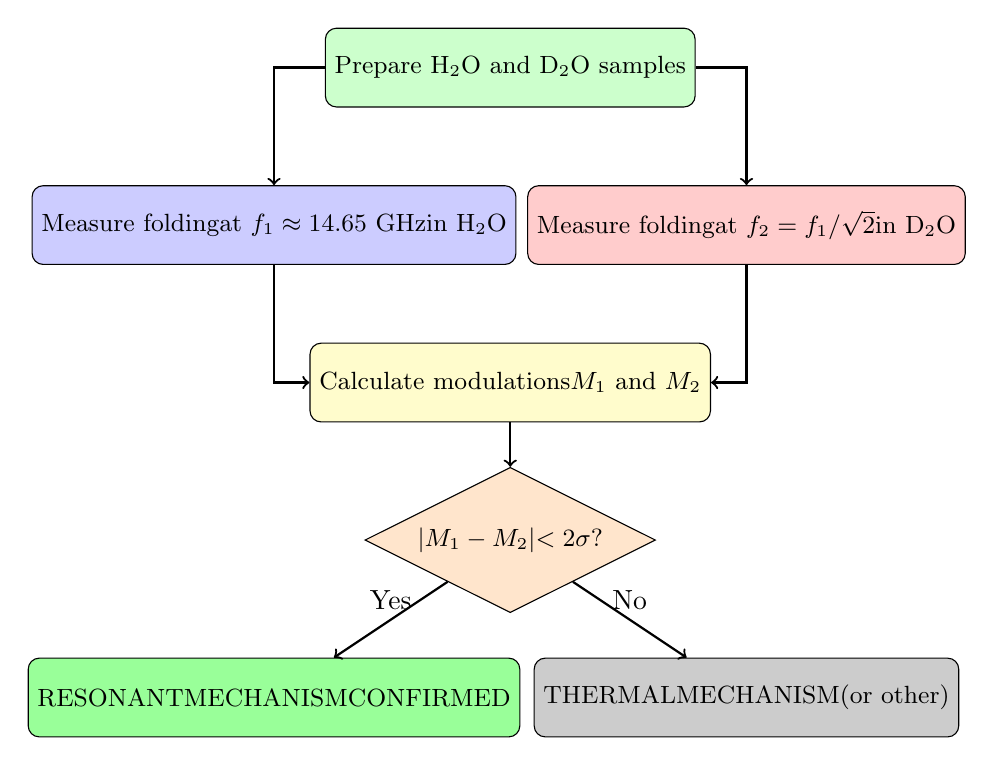
\begin{tikzpicture}[
    block/.style={rectangle, draw, rounded corners, minimum width=3cm, minimum height=1cm, text centered, font=\small},
    decision/.style={diamond, draw, minimum width=2cm, minimum height=1cm, text centered, font=\small, aspect=2},
    arrow/.style={->, thick}
]
    % Start
    \node[block, fill=green!20] (start) at (0,8) {Prepare H$_2$O and D$_2$O samples};
    
    % H2O measurement
    \node[block, fill=blue!20] (h2o) at (-3,6) {Measure folding\\at $f_1 \approx 14.65$ GHz\\in H$_2$O};
    
    % D2O measurement
    \node[block, fill=red!20] (d2o) at (3,6) {Measure folding\\at $f_2 = f_1/\sqrt{2}$\\in D$_2$O};
    
    % Calculate modulations
    \node[block, fill=yellow!20] (calc) at (0,4) {Calculate modulations\\$M_1$ and $M_2$};
    
    % Decision
    \node[decision, fill=orange!20] (decide) at (0,2) {$|M_1 - M_2|$\\$< 2\sigma$?};
    
    % Outcomes
    \node[block, fill=green!40] (resonant) at (-3,0) {RESONANT\\MECHANISM\\CONFIRMED};
    \node[block, fill=gray!40] (thermal) at (3,0) {THERMAL\\MECHANISM\\(or other)};
    
    % Arrows
    \draw[arrow] (start) -- (-3,8) -- (h2o);
    \draw[arrow] (start) -- (3,8) -- (d2o);
    \draw[arrow] (h2o) -- (-3,4) -- (calc);
    \draw[arrow] (d2o) -- (3,4) -- (calc);
    \draw[arrow] (calc) -- (decide);
    \draw[arrow] (decide) -- node[above] {Yes} (resonant);
    \draw[arrow] (decide) -- node[above] {No} (thermal);
    
\end{tikzpicture}
\caption{Flowchart of the isotope verification protocol}
\label{fig:flowchart}
\end{figure}

\subsection{Expected Results}

\subsubsection{Resonant Mechanism (Predicted Outcome)}

If the effect is due to resonant coupling to the molecular gate:

\begin{enumerate}[label=(\arabic*)]
\item Folding rate reduction observed at $f_1 \approx 14.65$ GHz in H$_2$O.
\item Folding rate reduction of \textbf{equal magnitude} observed at $f_2 \approx 10.4$ GHz in D$_2$O.
\item Frequency ratio $f_1/f_2 = \sqrt{2}$ within experimental uncertainty.
\item Irradiating H$_2$O at 10.4 GHz produces \textbf{no effect}.
\item Irradiating D$_2$O at 14.65 GHz produces \textbf{no effect}.
\end{enumerate}

\subsubsection{Thermal Mechanism (Alternative Outcome)}

If the effect is purely thermal:

\begin{enumerate}[label=(\arabic*)]
\item Effects observed over a broad frequency range in both solvents.
\item Optimal frequencies differ by $<$25\% (dielectric shift), not 41\%.
\item Effects correlate with temperature rise, not specific frequency.
\item Cross-irradiation (H$_2$O at D$_2$O frequency or vice versa) produces partial effects proportional to dielectric absorption.
\end{enumerate}

\begin{figure}[h]
\centering
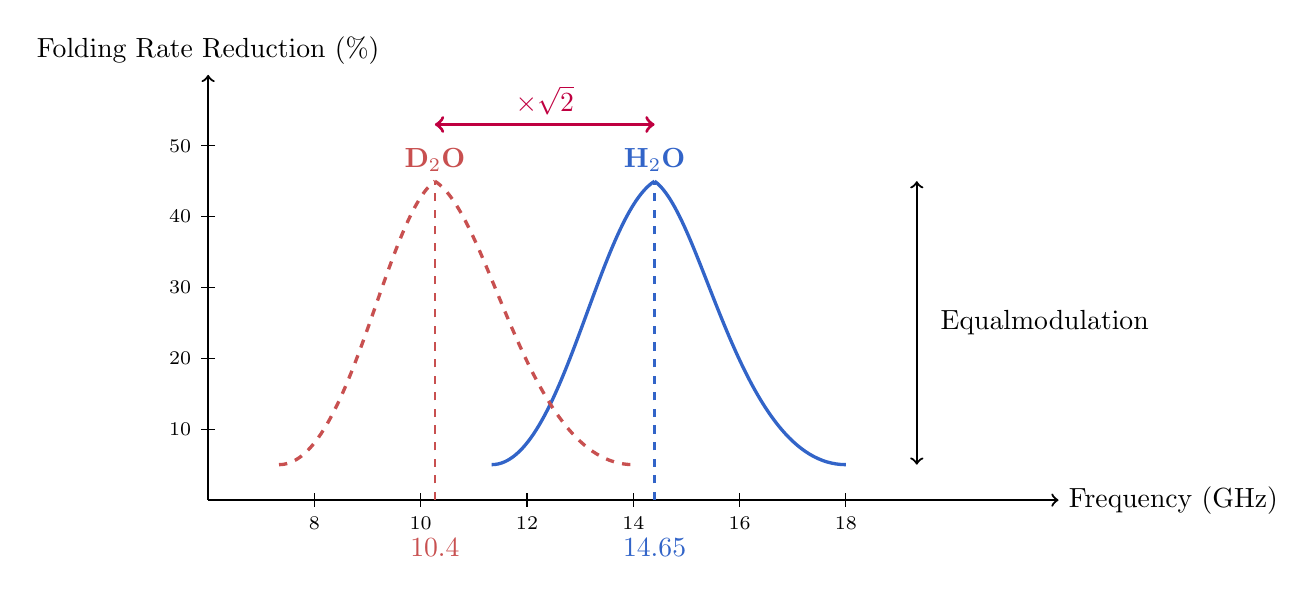
\begin{tikzpicture}[scale=0.9]
    % Axes
    \draw[thick,->] (0,0) -- (12,0) node[right] {Frequency (GHz)};
    \draw[thick,->] (0,0) -- (0,6) node[above] {Folding Rate Reduction (\%)};
    
    % Axis labels
    \foreach \x/\label in {1.5/8, 3/10, 4.5/12, 6/14, 7.5/16, 9/18} {
        \draw (\x,0.1) -- (\x,-0.1) node[below] {\scriptsize \label};
    }
    \foreach \y/\label in {1/10, 2/20, 3/30, 4/40, 5/50} {
        \draw (0.1,\y) -- (-0.1,\y) node[left] {\scriptsize \label};
    }
    
    % H2O resonance (at 14.65 GHz)
    \draw[very thick, h2o] (4,0.5) .. controls (5,0.5) and (5.5,4) .. (6.3,4.5);
    \draw[very thick, h2o] (6.3,4.5) .. controls (7,4) and (7.5,0.5) .. (9,0.5);
    \node[h2o, above] at (6.3,4.5) {\textbf{H$_2$O}};
    
    % D2O resonance (at 10.4 GHz)
    \draw[very thick, d2o, dashed] (1,0.5) .. controls (2,0.5) and (2.5,4) .. (3.2,4.5);
    \draw[very thick, d2o, dashed] (3.2,4.5) .. controls (4,4) and (4.5,0.5) .. (6,0.5);
    \node[d2o, above] at (3.2,4.5) {\textbf{D$_2$O}};
    
    % Markers
    \draw[h2o, thick, dashed] (6.3,0) -- (6.3,4.5);
    \node[h2o, below] at (6.3,-0.4) {14.65};
    
    \draw[d2o, thick, dashed] (3.2,0) -- (3.2,4.5);
    \node[d2o, below] at (3.2,-0.4) {10.4};
    
    % Arrow showing sqrt(2) shift
    \draw[<->, very thick, purple] (3.2,5.3) -- (6.3,5.3);
    \node[purple, above] at (4.75,5.3) {$\times\sqrt{2}$};
    
    % Equal modulation
    \draw[<->, thick, black] (10,4.5) -- (10,0.5);
    \node[right] at (10.2,2.5) {Equal\\modulation};
    
\end{tikzpicture}
\caption{Expected resonance curves showing equal modulation at $\sqrt{2}$-shifted frequencies}
\label{fig:resonance}
\end{figure}

\subsection{Control Experiments}

\subsubsection{Essential Controls}

\begin{enumerate}[label=(\arabic*)]
\item \textbf{No-irradiation control:} Folding kinetics without microwave irradiation in both H$_2$O and D$_2$O.

\item \textbf{Off-resonance control:} Irradiation at frequencies well away from predicted resonances (e.g., 8 GHz in H$_2$O, 6 GHz in D$_2$O).

\item \textbf{Cross-irradiation control:}
\begin{itemize}
\item H$_2$O at D$_2$O frequency (10.4 GHz)---should show no effect if resonant.
\item D$_2$O at H$_2$O frequency (14.65 GHz)---should show no effect if resonant.
\end{itemize}

\item \textbf{Temperature control:} Conventional heating to same temperature rise observed during irradiation---should not reproduce the effect if resonant.
\end{enumerate}

\subsubsection{Additional Validation Experiments}

\begin{enumerate}[label=(\arabic*)]
\item \textbf{Partial deuteration:} Measure effects at intermediate H$_2$O/D$_2$O mixtures. Resonant frequency should shift proportionally.

\item \textbf{Different proteins:} Verify that the optimal frequencies are the same for different proteins (universal molecular gate).

\item \textbf{Power titration:} Vary power at fixed frequency to characterize dose-response.
\end{enumerate}

\subsection{Decision Matrix}

\begin{table}[h]
\centering
\begin{tabular}{p{0.35\textwidth}cc}
\toprule
\textbf{Observation} & \textbf{Resonant} & \textbf{Thermal} \\
\midrule
$f_1/f_2 = \sqrt{2} \pm 5\%$ & \checkmark & $\times$ \\
$M_1 \approx M_2$ at predicted frequencies & \checkmark & $\times$ \\
Sharp resonance (FWHM $<$ 2 GHz) & \checkmark & $\times$ \\
Cross-irradiation shows no effect & \checkmark & $\times$ \\
Effect independent of power (above threshold) & \checkmark & $\times$ \\
Temperature rise correlates with effect & $\times$ & \checkmark \\
Broad frequency response & $\times$ & \checkmark \\
\bottomrule
\end{tabular}
\caption{Decision matrix for interpreting isotope verification results}
\label{tab:decision}
\end{table}

\subsection{Quantitative Predictions}

Based on the Recognition Science framework and machine-verified proofs:

\begin{table}[h]
\centering
\begin{tabular}{lll}
\toprule
\textbf{Parameter} & \textbf{Predicted Value} & \textbf{Uncertainty} \\
\midrule
H$_2$O jamming frequency $f_1$ & 14.65 GHz & (12, 17) GHz \\
D$_2$O jamming frequency $f_2$ & 10.37 GHz & (8, 13) GHz \\
Frequency ratio $f_1/f_2$ & $\sqrt{2} = 1.414$ & $\pm$5\% \\
Modulation magnitude (at resonance) & 30--50\% & Protein-dependent \\
Resonance width (FWHM) & $\sim$1--2 GHz & Protein-dependent \\
\bottomrule
\end{tabular}
\caption{Quantitative predictions for isotope verification experiment}
\end{table}

\subsection{Interpretation of Edge Cases}

\subsubsection{Case 1: Equal Modulation, Wrong Ratio}

If $M_1 \approx M_2$ but $f_1/f_2 \neq \sqrt{2}$:
\begin{itemize}
\item Possible resonant mechanism with different underlying oscillator.
\item Requires investigation of alternative coupling pathways.
\end{itemize}

\subsubsection{Case 2: Correct Ratio, Unequal Modulation}

If $f_1/f_2 = \sqrt{2}$ but $M_1 \neq M_2$:
\begin{itemize}
\item Possible resonant mechanism with different coupling strengths in H$_2$O vs.\ D$_2$O.
\item May indicate secondary effects of deuteration on protein dynamics.
\end{itemize}

\subsubsection{Case 3: Partial Isotope Effect}

If observed frequency shift is between 10\% (thermal) and 41\% (resonant):
\begin{itemize}
\item May indicate mixed mechanism (both thermal and resonant contributions).
\item Requires deconvolution of contributions.
\end{itemize}

\newpage

%% ============================================================================
%%                              CLAIMS
%% ============================================================================

\section{CLAIMS}

What is claimed is:

\subsection{Method Claims}

\begin{enumerate}[label=\textbf{\arabic*.}]

\item A method for verifying that modulation of protein folding rate by electromagnetic radiation is due to a resonant mechanism, comprising:
\begin{enumerate}[label=(\alph*)]
\item providing a first protein sample in H$_2$O-based solvent;
\item irradiating said first sample at a first frequency $f_1$ in the range of 12 to 17 GHz;
\item measuring a first folding rate modulation $M_1$;
\item providing a second protein sample in D$_2$O-based solvent;
\item irradiating said second sample at a second frequency $f_2 = f_1/\sqrt{2}$;
\item measuring a second folding rate modulation $M_2$; and
\item confirming a resonant mechanism if $|M_1 - M_2|$ is less than a predetermined threshold.
\end{enumerate}

\item The method of claim 1, wherein the predetermined threshold is two standard deviations of the experimental uncertainty.

\item The method of claim 1, wherein $f_1 \approx 14.65$ GHz and $f_2 \approx 10.4$ GHz.

\item The method of claim 1, wherein the frequency ratio $f_1/f_2$ equals $\sqrt{2}$ within $\pm$5\%.

\item The method of claim 1, further comprising a control experiment of irradiating the H$_2$O sample at frequency $f_2$ and confirming that no significant folding rate modulation occurs.

\item The method of claim 1, further comprising a control experiment of irradiating the D$_2$O sample at frequency $f_1$ and confirming that no significant folding rate modulation occurs.

\item The method of claim 1, wherein the folding rate modulation is measured by monitoring intrinsic tryptophan fluorescence during folding.

\item A method for determining the optimal frequency for resonant protein folding modulation, comprising:
\begin{enumerate}[label=(\alph*)]
\item performing a first frequency sweep in H$_2$O over a frequency range of 12 to 17 GHz;
\item identifying a first optimal frequency $f_1^*$ at which folding rate modulation is maximized;
\item performing a second frequency sweep in D$_2$O over a frequency range of 8 to 13 GHz;
\item identifying a second optimal frequency $f_2^*$ at which folding rate modulation is maximized; and
\item verifying that $f_1^*/f_2^* = \sqrt{2}$ within experimental uncertainty.
\end{enumerate}

\item The method of claim 8, wherein the frequency sweep comprises measuring folding rate at a plurality of frequencies spaced by 0.1 to 1.0 GHz.

\item The method of claim 8, further comprising refining the optimal frequency by performing a fine frequency sweep with frequency spacing of 0.01 to 0.1 GHz around the initially identified optimal frequency.

\item A method for discriminating between resonant and thermal mechanisms in electromagnetic modulation of protein folding, comprising:
\begin{enumerate}[label=(\alph*)]
\item measuring the frequency shift between optimal frequencies in H$_2$O and D$_2$O;
\item if said frequency shift is greater than 35\%, concluding that the mechanism is predominantly resonant;
\item if said frequency shift is less than 20\%, concluding that the mechanism is predominantly thermal; and
\item if said frequency shift is between 20\% and 35\%, concluding that the mechanism is mixed.
\end{enumerate}

\item The method of claim 11, wherein the expected frequency shift for a resonant mechanism is approximately 41\% (factor of $\sqrt{2}$).

\item The method of claim 11, wherein the expected frequency shift for a thermal mechanism is approximately 10--20\% based on dielectric property differences between H$_2$O and D$_2$O.

\item A method for validating the Recognition Science prediction of protein folding jamming frequency, comprising:
\begin{enumerate}[label=(\alph*)]
\item irradiating a protein sample in H$_2$O at approximately 14.65 GHz;
\item measuring folding rate modulation at said frequency;
\item irradiating an equivalent protein sample in D$_2$O at approximately 10.4 GHz;
\item measuring folding rate modulation at said frequency; and
\item confirming the Recognition Science prediction if both samples show equal folding rate modulation within experimental uncertainty.
\end{enumerate}

\item The method of claim 14, wherein the predicted frequencies are derived from the molecular gate timescale $\tau_{19} = \tau_0 \times \varphi^{19} \approx 68$ ps, where $\varphi = (1+\sqrt{5})/2$ is the golden ratio.

\end{enumerate}

\subsection{Diagnostic Claims}

\begin{enumerate}[label=\textbf{\arabic*.}]
\setcounter{enumi}{15}

\item A method for using isotope substitution as a diagnostic for resonant electromagnetic effects on biomolecules, comprising:
\begin{enumerate}[label=(\alph*)]
\item measuring a biological effect in H$_2$O at a first frequency $f_1$;
\item measuring the same biological effect in D$_2$O at a second frequency $f_2 = f_1/\sqrt{2}$;
\item if the effects are equal in magnitude, concluding that the mechanism involves hydrogen-containing oscillators; and
\item if the effects are unequal, concluding that the mechanism does not primarily involve hydrogen-containing oscillators.
\end{enumerate}

\item The method of claim 16, wherein the biological effect is protein folding rate modulation.

\item The method of claim 16, wherein the biological effect is enzyme activity modulation.

\item The method of claim 16, wherein the biological effect is membrane permeability modulation.

\end{enumerate}

\subsection{Claims Related to Protocol}

\begin{enumerate}[label=\textbf{\arabic*.}]
\setcounter{enumi}{19}

\item A protocol for performing an isotope verification experiment, comprising:
\begin{enumerate}[label=(\alph*)]
\item preparing a protein sample in H$_2$O buffer and an equivalent sample in D$_2$O buffer with $>$95\% H/D exchange;
\item measuring baseline folding rates for both samples without irradiation;
\item irradiating the H$_2$O sample at frequency $f_1 \in (12, 17)$ GHz and measuring modulated folding rate;
\item irradiating the D$_2$O sample at frequency $f_2 = f_1/\sqrt{2}$ and measuring modulated folding rate;
\item calculating modulation magnitudes $M_1$ and $M_2$ relative to baseline;
\item performing statistical comparison of $M_1$ and $M_2$; and
\item reporting whether the resonant mechanism criterion ($|M_1 - M_2| < 2\sigma$) is satisfied.
\end{enumerate}

\item The protocol of claim 20, further comprising control experiments selected from:
\begin{enumerate}[label=(\roman*)]
\item irradiation of H$_2$O at the D$_2$O frequency;
\item irradiation of D$_2$O at the H$_2$O frequency;
\item irradiation at off-resonance frequencies in both solvents; and
\item conventional heating to equivalent temperature rise.
\end{enumerate}

\end{enumerate}

\newpage

%% ============================================================================
%%                         ABSTRACT
%% ============================================================================

\section*{ABSTRACT}
\addcontentsline{toc}{section}{ABSTRACT}

A method for verifying that modulation of protein folding rates by electromagnetic radiation is due to a resonant mechanism rather than thermal heating. The method exploits the characteristic $\sqrt{2}$ isotope shift between H$_2$O and D$_2$O that arises from the mass dependence of molecular oscillation frequencies ($f \propto 1/\sqrt{m}$). The method comprises: performing a first measurement of folding rate modulation in H$_2$O at a frequency $f_1$ in the range 12--17 GHz (preferably $\sim$14.65 GHz); performing a second measurement in D$_2$O at frequency $f_2 = f_1/\sqrt{2}$ (range 8--13 GHz, preferably $\sim$10.4 GHz); and confirming the resonant mechanism if the modulation magnitudes are equal within experimental uncertainty. The 41\% frequency shift ($\sqrt{2}$) is characteristic of a resonant mechanism coupling to hydrogen-containing oscillators, whereas thermal effects show at most a 10--20\% shift due to dielectric property differences. Control experiments (cross-irradiation, off-resonance) provide additional confirmation. The method provides an unambiguous ``smoking gun'' signature for discriminating between resonant and thermal mechanisms, with quantitative predictions verified by machine-checked proofs. Applications include validation of Recognition Science predictions, characterization of electromagnetic bioeffects, and quality control for resonant protein folding modulation therapies.

\vspace{1in}

\begin{center}
\textbf{--- END OF SPECIFICATION ---}
\end{center}

\newpage

%% ============================================================================
%%                         INVENTOR DECLARATION
%% ============================================================================

\section*{INVENTOR DECLARATION}
\addcontentsline{toc}{section}{INVENTOR DECLARATION}

I, Jonathan Washburn, declare that:

\begin{enumerate}[label=(\arabic*)]
\item I am the original and sole inventor of the method described and claimed in this application.

\item I have reviewed the above specification and claims and believe them to be accurate and complete.

\item I believe the claimed invention to be novel, useful, and non-obvious over the prior art.

\item I authorize the filing of this provisional patent application to establish a priority date.
\end{enumerate}

\vspace{1in}

\noindent\textbf{Inventor Signature:} \hrulefill

\vspace{0.5in}

\noindent\textbf{Name:} Jonathan Washburn

\noindent\textbf{Email:} washburn.jonathan@gmail.com

\noindent\textbf{Date:} \hrulefill

\vspace{1in}

\begin{center}
\textit{This document is intended for provisional patent application filing purposes.\\
All information contained herein is confidential and proprietary.}
\end{center}

\end{document}
